% ORIGINAL FIGURE. The arbitration rule THIS SYSTEM implements, plotted from
% its own constants, beside the continuous blend it deliberately does not use.
% Drawn from the implementation, not copied from a published figure.
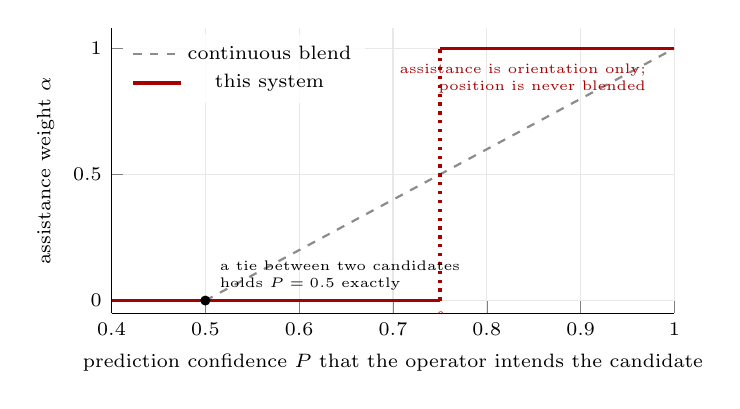
\begin{tikzpicture}
\begin{axis}[
    width=0.72\linewidth, height=52mm,
    xmin=0.4, xmax=1.0, ymin=-0.05, ymax=1.08,
    xlabel={prediction confidence $P$ that the operator intends the candidate},
    ylabel={assistance weight $\alpha$},
    xlabel style={font=\scriptsize}, ylabel style={font=\scriptsize},
    tick label style={font=\scriptsize},
    legend style={font=\scriptsize, at={(0.02,0.98)}, anchor=north west,
                  draw=none, fill=white, fill opacity=0.85, text opacity=1},
    axis lines*=left, grid=major, grid style={gray!18},
]
% continuous blend: alpha rises with confidence from the tie point
\addplot[black!45, thick, dashed, domain=0.5:1.0, samples=60]
  {(x-0.5)/0.5};
\addlegendentry{continuous blend}
% this system: a threshold, and nothing below it
\addplot[red!65!black, very thick] coordinates {(0.4,0) (0.75,0)};
\addlegendentry{this system}
\addplot[red!65!black, very thick] coordinates {(0.75,1) (1.0,1)};
\addplot[red!65!black, very thick, dotted] coordinates {(0.75,0) (0.75,1)};
\addplot[only marks, mark=*, mark size=1.6pt, black]
  coordinates {(0.5,0)};
\node[font=\tiny, anchor=west, align=left] at (axis cs:0.505,0.10)
  {a tie between two candidates\\holds $P=\num{0.5}$ exactly};
\node[font=\tiny, anchor=north, red!65!black] at (axis cs:0.75,-0.005)
  {$\theta$};
\node[font=\tiny, anchor=east, align=right, red!65!black]
  at (axis cs:0.98,0.88) {assistance is orientation only;\\position is never blended};
\end{axis}
\end{tikzpicture}
